\documentclass[a4paper, 10pt, final, garamond]{book}
\usepackage{cours-preambule}

\raggedbottom

\makeatletter
\renewcommand{\@chapapp}{Programme de kh\^olle -- semaine}
\makeatother

\begin{document}
\setcounter{chapter}{14}

\chapter{Du 16 au 20 janvier}

\section{Cours et exercices}
\section*{Ondes chapitre 2 -- Interférences à deux ondes}
\begin{enumerate}[label=\Roman*]
    \item \textbf{Rappel déphasages}~: définition, valeurs particulières,
        lecture graphique.
    \item \textbf{Superposition d'ondes sinusoïdales de mêmes fréquences}~:
        introduction, signaux de même amplitude, signaux d'amplitudes
        différentes, bilan.
    \item \textbf{Approximation par une onde plane}~: sources ponctuelles,
        différence de marche, exercice d'application.
    \item \textbf{Interférences lumineuses}~: cohérence, intensité, formule de
        \textsc{Fresnel}, chemin optique.
    \item \textbf{Expérience des trous d'\textsc{Young}}~: introduction,
        présentation, détermination de l'interfrange.
\end{enumerate}

\section{Cours uniquement}
\section*{Mécanique chapitre 1 -- Cinématique du point}
\begin{enumerate}[label=\Roman*]
    \item \textbf{Système et point matériel}~: définition système, point
        matériel.
    \item \textbf{Description et paramétrage du mouvement}~: notion de
        référentiel, relativité du mouvement, exemples de référentiels, vecteur
        base de projection et repère.
    \item \textbf{Position, vitesse et accélération}~: position et déplacement
        élémentaire, équations horaires et trajectoires~; vitesse et vitesse
        instantanée, notation pointée~; accélération et accélération
        instantanée.
    \item \textbf{Exemples de mouvements}~: rectiligne uniforme, rectiligne
        uniformément accéléré, courbe uniformément accéléré.
\end{enumerate}

\section*{Mécanique chapitre 2 -- Dynamique du point}
\begin{enumerate}[label=\Roman*]
    \item \textbf{Introduction}~: inertie et quantité de mouvement, forces
        fondamentales.
    \item \textbf{Trois lois de \textsc{Newton}}~: principe d'inertie, principe
        fondamental de la mécanique, loi des actions réciproques.
    \item \textbf{Systèmes de points}~: centre d'inertie, quantité de mouvement
        d'un ensemble de points, théorème de la résultante cinétique.
    \item \textbf{Méthode générale de résolution}.
    \item \textbf{Le poids}~: définition, chute libre avec angle initial.
    \item \textbf{Poussée d'\textsc{Archimède}}.
    \item \textbf{Frottement fluide}~: force de frottement fluide, chute libre
        sans vitesse initiale avec frottements linéaires, avec frottements
        quadratique, résolution par adimensionnement.
\end{enumerate}

\section{Questions de cours possibles}
\begin{enumerate}
    \item Refaire l'exercice~:
\end{enumerate}
\begin{NCexem}[breakable]{Exercice}
    \begin{minipage}{0.55\linewidth}
        Soient 2 émetteurs sonores envoyant une onde progressive sinusoïdale de
        même fréquence, amplitude et phase à l'origine. Le premier est fixé à
        l'origine du repère, l'émetteur 2 est mobile et à une distance $d$ du
        premier, et un microphone est placé à une distance fixe $x_0$ de
        l'émetteur 1 et est aligné avec les deux émetteurs. On néglige
        l'influence de l'émetteur 2 sur l'émetteur 1 et toute atténuation.
    \end{minipage}
    \hfill
    \begin{minipage}{0.45\linewidth}
        \begin{center}
            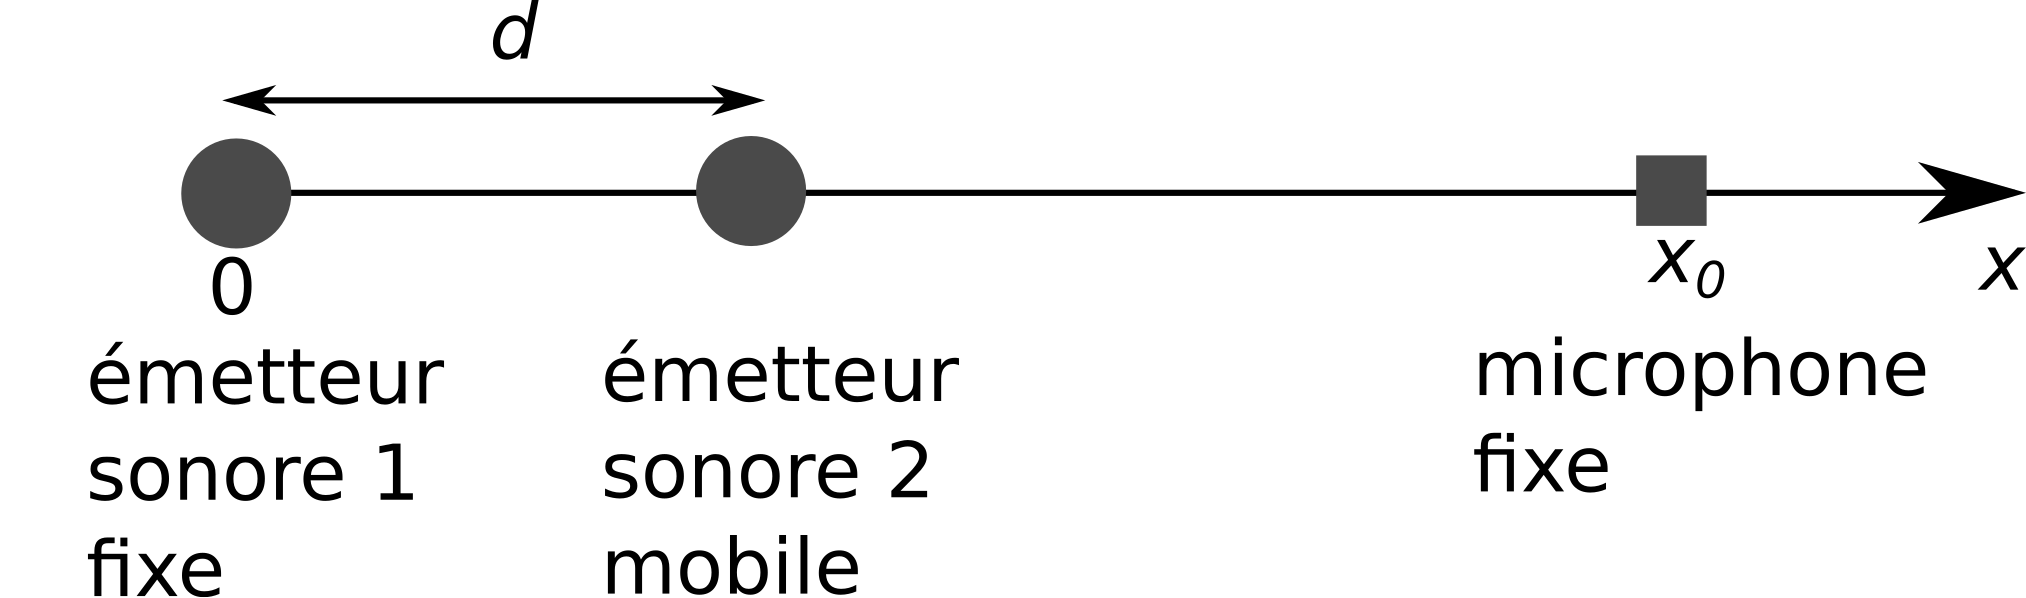
\includegraphics[width=\linewidth]{microphone}
        \end{center}
    \end{minipage}
    \begin{enumerate}[label=\sqenumi]
        \item Lorsque $d=0$, qu'enregistre-t-on au niveau du microphone~?
        \item On part de $d=0$ et on augmente $d$ jusqu'à ce que le signal
            enregistré soit nul. Ceci se produit pour $d = \SI{6.0}{cm}$.
            Expliquer cette extinction.
        \item En déduire la longueur d'onde du son émis.
        \item Pour $d = \SI{12.0}{cm}$, quelle sera l'amplitude du signal
            enregistré~?
    \end{enumerate}
\end{NCexem}
\begin{enumerate}[resume]
    \item Déterminer l'expression du signal somme de deux ondes sinusoïdales de
        même fréquence \textbf{et même amplitude} en introduisant $\Delta
        \f(\Mr)$ et $\f_0(\Mr)$. Définir et \textbf{déterminer}, donc
        \textbf{calculer} son intensité lumineuse. On la mettra sous la forme de
        la formule de \textsc{Fresnel}. Exprimer les valeurs de $\D\f(\Mr)$
        correspondant à des interférences constructives ou destructives.
        On pourra redonner
        \[\cos p + \cos q =
            2\cos \left( \frac{p+q}{2} \right)\cos \left( \frac{p-q}{2} \right)\]
    \item Démontrer le lien entre déphasage et différence de marche. Démontrer
        le lien entre déphasage et chemin optique. Donner les déphasages pour
        lesquels on a des interférences constructives et destructives.
        Déterminer les différences de chemin optique correspondant.
    \item Trous d'\textsc{Young}~: présenter l'expérience et montrer que la
        différence de chemin $\delta_{2/1}(\Mr)$ s'écrit \hfill $\delta =
        2ax/D$ avec $2a$ la distance entre les fentes. Donner les conditions sur
        $x$ pour avoir interférences constructives ou destructives. \smallbreak
        On pourra redonner
        \[\sqrt{1+\ep} = 1 + \ep/2 + o(\ep)\]
    \item Déterminer les équations horaires du mouvement rectiligne uniformément
        accéléré. Un attention particulière sera portée à l'établissement du
        système d'étude.
    \item Déterminer les équations horaires du mouvement courbe uniformément
        accéléré avec $\vf_0$ faisant un angle $\alpha$ avec l'horizontale. Une
        attention particulière sera portée à l'établissement du système d'étude.
    \item Pour un mouvement courbe uniforme accéléré avec $\vf(0) =
        v_0\cos\alpha\ux + v_0\sin\alpha\uy$, à partir de
        \[ \left\{
                \begin{array}{l}
                    x(t) = v_0t\cos\alpha\\
                    y(t) = -\frac{1}{2}gt^2 + v_0t \sin\alpha
                \end{array}
            \right.
        \]
        déterminer la portée, la flèche du tir ainsi que le temps de vol.
    \item Déterminer la proportion immergée d'un glaçon. On donne $\rho_{\rm
        eau} = \SI{1.00e3}{km.m^{-3}}$ et $\rho_{\rm glace} =
        \SI{9.17e2}{kg.m^{-3}}$.

    \item Déterminer la vitesse limite et le temps caractéristique du mouvement
        pour une chute libre sans vitesse initiale avec frottements linéaires.
        Une approche d'adimensionnement d'équation différentielle, de solution
        particulière ou de résolution totale directe est possible.
\end{enumerate}

\end{document}
